\section{Návrh metódy}
Navrhovaná metóda zohľadnuje vlastnosti ktoré nie je možné získať iba zo statického obrazu, budeme ich nazívať dynamické príznaky videa.
Avšak metóda stále zohľadnuje v pozorovanom videu aj aspekty statického obrazu, tieto budeme nazívať statické príznaky videa.
Tieto príznaky sú vypočítavané seprátne a nakoniec ich metóda spája do jednej výslednej mapy pozornosti. Výsledkom je postupnosť máp pozornosti pre každý frame videa (podľa vstupnej konfigurácie), ktorý možno spojiť do videa pozornosti pre ľubovolné vstupné video.

\subsection{Dynamické príznaky videa}
Dynamické príznaky metóda najprv extrahuje pomocou štadardnej metódy Horn-Schunck, (referencia na 2 kapitolu alebo na článok?) ktorá vypočíta optický tok na každých 2 rozdielnych framoch videa čím vzniká sémantický príznak pohybu rôznych objektov po scéne spolu s smerovýmy vektormy pohybu daných vektorov.
Získané smerové vektory okamžite spočítavame aby sme získali celkový obraz optického toku pre danú dvojicu obrazov.
Obraz sa následne prahuje statickou konštantou kôli ostráneniu šumu.
Prahovanie prebieha dynamicky vzľadom na počet nájdených 8-spojitých regiónov tj. výstup optikého toku. V našej implementácií je obmedzený počet regiónov na maximálnu hodnotu 200 regiónov.
Prahovanie začne s konštantou ktorú určí pomocou algoritmu Otsu\cite{otsu}, následne určí počet 8-spojitých regiónov akje počet vädší ako maximálna hodnota, zvýši konštantu o 10% z pôvodnej hodnoty.
Tento proces sa opakuje pokial sa v obraze vyskytuje viacej ako maximálny počet regiónov.
Takéto prahovanie je nutné pre optimalizáciu výkonu algoritmu, pretože v prípadoch ked obraz obsahuje veľké množtvo regónov výpočtová rýchlosť algortmu je maximálne neúčinná.
Pixeli s valídnou honotou sa rozdelia na regióny podľa spojitosti a podobnosti štandardným spôsobom.
Pripomenme, že v tomto obraze sa spočítali hodnoty posunu v oboch smeroch aritmeticky do jednej hodnotiacej konštanty (pre každý pixel obrazu), ktorá už nereprezentuje smer posunu daného obrazového pixelu, ale iba hodnotí celkový posun pixelu.
Takto získané regóny budeme vyhodnocovať a spájať podľa pôvodných výsledkov metódy Horn-Schunck.
Vďaka využitiu pôvodných vektorov z výsledku metódy Horn-Schunck, vieme rozlíšiť pohyb horizontálny aj vertikálny separátne.
Pre všetky dvojice regiónov v obraze zistujeme nasledovné charakteristiky:
\begin{enumerate}
  \item\textbf{Rozdiel smerových vektorov v horizontálnom smere}
  \item\textbf{Rozdiel smerových vektorov v vertikálnom smere}
  \item\textbf{Rozdiel vo vzdialenosti}
\end{enumerate}
\subsubsection{Rozdiel smerových vektorov v horizontálnom smere}
Charakteristika sa vypočítava zo smerových horizontálnych vektorov metódy Horn-Schunck.
Pre každý región sa vypočíta maximálna hodnota z indexov daného regiónu.
Následne sa za hodnotu chrakteristiky sa považuje absolútna hodnota rozdielu týchto hodnôt pre každý región.
\begin{equation}
  H_A = max(HS(i_A))
\end{equation}
\begin{equation}
  H_B = max(HS(i_B))
\end{equation}
\begin{equation}
  R_{H} = abs(H_A-H_B)
\end{equation}
Kde A, B reprezentuju všetky dvojice regiónov ktoré sa nachádzajú v obraze.
\begin{math}V_a, V_b\end{math} je maximálna hodnota horizontálnych smerových vektorov z výsledku Horn-Schunck algoritmu pre všetky oblasti patriace danému regiónu.
\begin{math}R_{H}\end{math} je výsledná hodnota charakteristiky.

\subsubsection{Rozdiel smerových vektorov v vertikálnom smere}
Charakteristika sa vypočítava zo smerových vertikálnych vektorov metódy Horn-Schunck.
Prekazdý región sa vypočíta maximálna hodnota z indexov daného regiónu.
Následne sa za hodnotu chrakteristiky sa považuje absolútna hodnota rozdielu týchto hodnôt.

\begin{equation}
  H_A = max(HS(i_A))
\end{equation}
\begin{equation}
  H_B = max(HS(i_B))
\end{equation}
\begin{equation}
  R_{V} = abs(H_A-H_B)
\end{equation}
Kde A, B reprezentuju všetky dvojice regiónov ktoré sa nachádzajú v obraze.
\begin{math}V_a, V_b\end{math} je maximálna hodnota verikálnych smerových vektorov z výsledku Horn-Schunck algoritmu pre všetky oblasti patriace danému regiónu.
\begin{math}R_{V}\end{math} je výsledná hodnota charakteristiky.

\subsubsection{Rozdiel vo vzdialenosti}
Chrakteristika sa vypočítava ako minimálna hodnota vzdialenosti medzi dvojicou regiónov.
Hodnota je počítaná euklidovskou metódou.

\begin{figure}[H]
  \begin{algorithm}[H]
   \ForAll{rohA ako každý extrém regiónu A}{
     \ForAll{rohB ako každý extrém regiónu b}{
      vzdialenost = sqrt( (corner2(1,1)-rohB(1,1))^2 + (rohB(1,2)-rohA(1,2))^2 ) \\
     }
   }
   \caption{Výpočet minimálnej vzdialenosti euklidovskou metódou}
  \end{algorithm}
  \vspace{10mm}
\end{figure}

\subsubsection{Spájanie regiónov}
Po výpočte všetkých 3 charakteristík spojíme všetky dovjice regionov, pre ktoré su všetky chrakteristyky nižšie ako zadefinovaná konštanta.
Regióny spájame pomocou konvexného obalu zjednotenia bodov ležiacich v oboch regiónoch.
\begin{figure}[H]
  \centering
  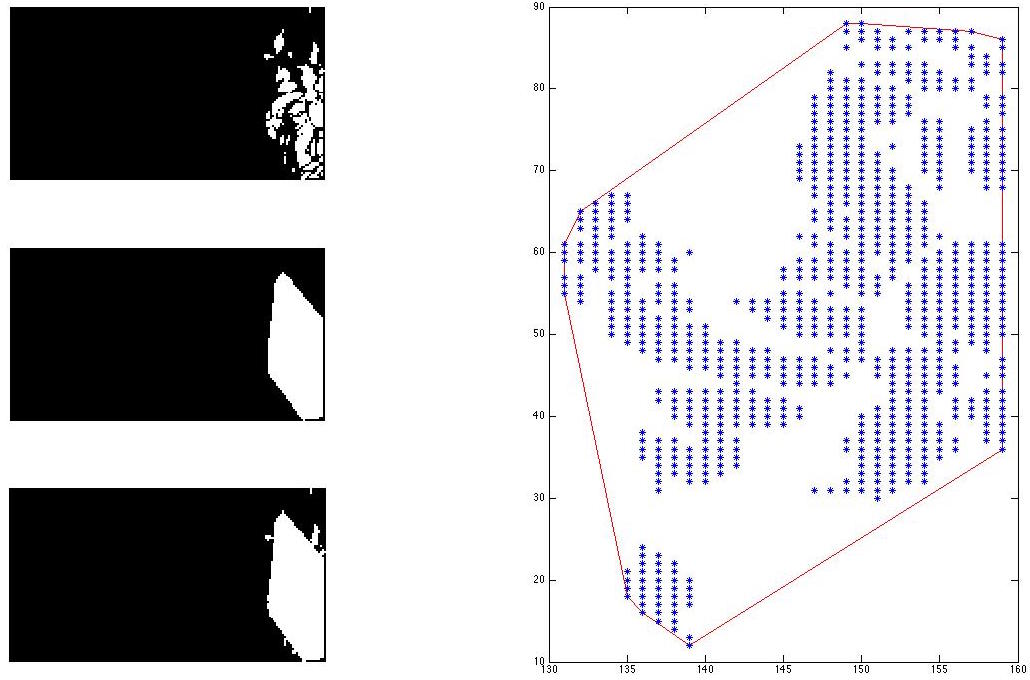
\includegraphics[width=15cm]{pics/spojenie-regionov.jpg}
  \caption{Vyzualizácia spojenia regiónov pomocou konvexného obalu}
  \vspace{10mm}
\end{figure}

\subsubsection{Starnutie objektov na scéne}
Do vypočitavnia dynamických príznakov započítavame predpoklad, že aj pohybujúce sa objekty postupne strácajú pozornosť používateľov.
A to v prípade kedy sa síce daný objekt na scéne pohybuje, ale na identickom mieste.
do metóty zabudujeme mechanizmus kde pixelom s dlhodobo vysokým hodnotením pozornosti, zmenšíme toto hodnotenie pomocou  vynásobenia koeficientom hodnoty \numrange{0}{1}.

\subsection{Statické príznaky videa}
Pri videách kde sa pohybuje celá scéna (kamera je v pohybe) nedávajú dynamické príznaky dobré výsledky kdeže logicky označia celú scénu alebo jej vädšinovú časť scény za výrazne salientnú.
Preto je vhodné dynamické príznaky vhodne kombinovať s klasickýmy modelmy pozornosti ktoré síce zanedbajú postupnosť obrazov, ale nezlyhajú ako dynamické príznaky.
Pre extrakciu statických obrázkov sme zvolili metódu založnú na spektralnych reziduach\cite{spectral-rezidual}.
Vďaka svojmu príncípu potlačovania štatisticky opakujúcich sa predmetov na scéne, sa dá predpokladaď vhodné doplnenie statických objektov ktoré možu zaujať pozornosť na videu ak zlyhávajú dynamické príznaky.

\subsection{Výsledné spojenie príznakov}
Spájanie dynamických a statických príznakov bude prebiehat pomocou sčítania oboch máp, pričom vždy s použijú v určitom pomere.
Výpočet pomeru bude určovať pomer výskytu salientných pixelov v mape dynamických príznakov.

@TODO add latex som symbol \\
\begin{equation}
  pomer = (sum(P_D} > 0))/Pix_{count}
\end{equation}
Kde \begin{math}P_D\end{math} reprezentuje mapu dynamických príznakov a \begin{math}Pix_{count}\end{math} je počet všetkých pixelov ktoré obraz obsahuje.

Ak je vysoký výskyt salientých pixelov, potrebujeme utlmit zobrazovanie tejto časti príznakov a prioritizovať zobrazovanie statických priznakov preto zmiešavacia funkcia vyzerá nasledovne:

\begin{equation}
  Výsledok = (P_D * (1-pomer)) + (P_S * pomer)
\end{equation}
Kde \begin{math}P_D\end{math} reprezentuje mapu dynamických príznakov a \begin{math}P_S\end{math} mapu statických príznakov.

V prípade, že algoritmus nedokáže detekovať žiadny pohyb na scéne, bol by model pozornosti prázdny.
Preto v prípade keď je vyššie spomýnaný pomer dynamických pixelov extrémne nízky použijeme ako výstup algoritmu iba statické príznaky.
Naopak v prípade, že kamera je v pohybe Horn-Schunck algoritmus označí ako pohybujúci sa vädšinovú oblasť obrazu a v tom prípade je potrebné utlmiť dynamické príznaky obrazu a do popredia vystupujú statické.

@TODO add new page symbol latex
\subsection{Pipeline metódy}
  Grafický popis metódy

  \begin{figure}[H]
    \centering
    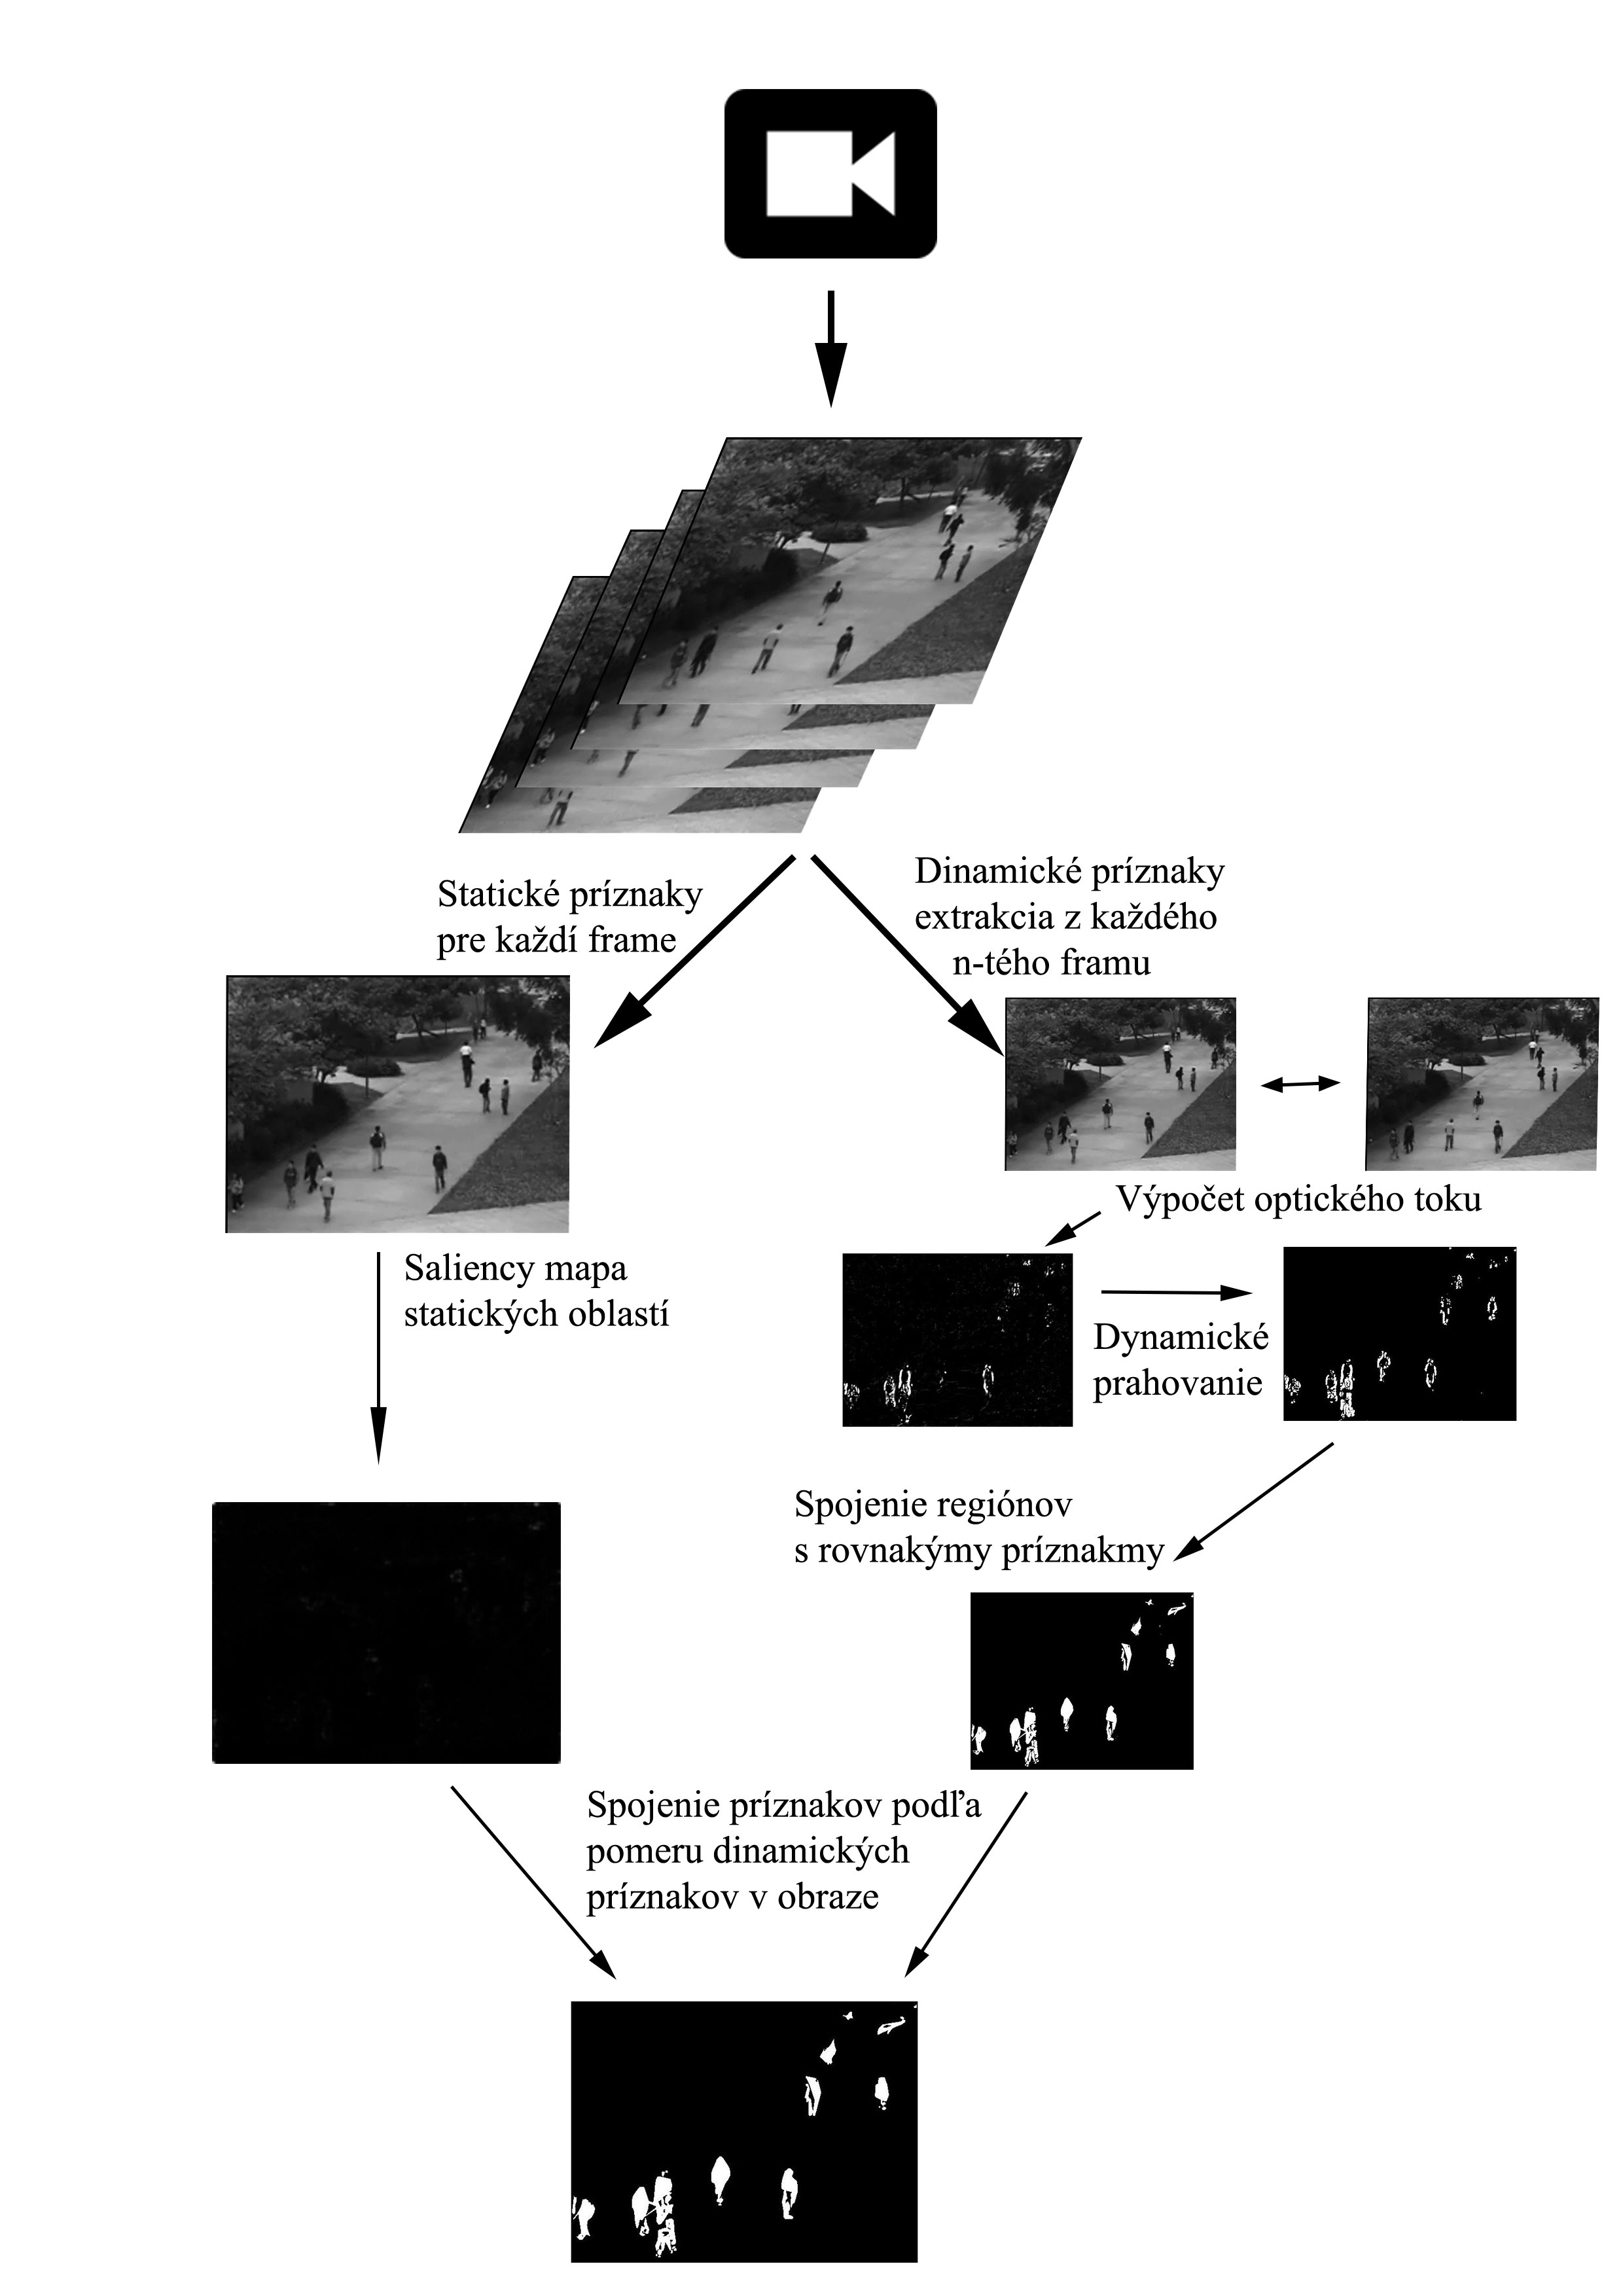
\includegraphics[width=15cm]{pics/workflow.jpg}
    \caption{Ucelená vyzualizácia algoritmu}
    \vspace{10mm}
  \end{figure}

\section{Implementácia riešenia}
Implementácia vyššie uvedeného algoritmu je implementovaná ako modul pre aplikáciu na porovnávanie a  automatickú validáciu výsledkov.
Aplikácia na porovnávanie je takisto implementovaná v prostredí matlab.

\subsection{Aplikáciu na porovnávanie a automatickú validáciu}
Sekundárnym prínosom práce je vytvorenie aplikácie pre zjednodušenie budúcej práce pri prototypovaní nových modelov pozornosti.
A následné uľahčenie validačného procesu pre potencionálnych vývojárov.\\
Základná functionalita:
\begin{enumerate}
  \item\textbf{Oddelenie logiky testovnia a logiky samotného modelu}
  \item\textbf{Simultálne sledovanie videa z viacerých modelov}
  \item\textbf{Spustenie a prezentovanie validácie}
  \item\textbf{Vizualizácia výsledkov validácie}
\end{enumerate}

\subsubsection{Oddelenie logiky testovnia a logiky samotného modelu}
\subsubsection{Simultálne sledovanie videa z viacerých modelov}
\subsubsection{Spustenie a prezentovanie validácie}
\subsubsection{Vizualizácia výsledkov validácie}

\subsection{Implementácia modulu}

\section{Validácia výsledkov}
Automatická validácia je možná pomocou datasetu\cite{accv}, ktorí bol upravený pre použitie s lubovolným modelom intregovaním do tejto applikácie.
\section{Možnosti pre zlepšenie}
\section{Diskusia}
